\section{Vector measures}

We can generalize the notion of complex measures, and finite real and positive measures through the notion of a vector measure, with most of the theory applying to vector measures as well. The following is mostly based on Søren Eilers' notes \cite{BergEilers} %%%%%%%%%%% Citer de rigtige sider
and also a bit on Halmos' notes \cite{Halmos}.


%%%%%%%%%%%%%%%%   DEFINITION OF VECTOR MEASURES   %%%%%%%%%%%%%%%%

\begin{definition} %%%%%%%% Revider
A vector measure on a measurable space $(X, \m{A})$, is a set function $\mu:\m{A} \to \R^{n}$ which is countably additive, i.e. an $n$-dimensional vector with finite real measures in every coordinate:
\begin{align*}
	\mu=(\mu_{1}, \dots, \mu_{n})
\end{align*}
and thus $\mu$ is countably additive if and only if all the $\mu_{i}$'s are so.
\end{definition}


%%%%%%%%%%%%%%%% DISCUSSION OF THE 1-NORM %%%%%%%%%%%%%%%%

We equip $\R^{n}$ with the 1-norm, and define the \textbf{absolute value} of $\mu$ as
\begin{align*}
	| \mu | (A) = \sup \left\{ \sum_{i=1}^{\infty} \n{\mu(A_{i})}_{1} \middle| \{ A_{i} \}_{i\in \N} \text{ is a partition of } A \right\}.
\end{align*}
Equipping $\R^{n}$ with the 1-norm has the advantage that
\begin{align}
	|\mu | = \sum_{i=1}^{n} |\mu_{i}| \label{eq: one norm}
\end{align}
where $|\mu_{i}|$ are the usual absolute values taken in $\R$. To see this, we note that
\begin{align*}
	\sum_{i=1}^{\infty} \n{\mu(A_{i})}_{1} = \sum_{j=1}^{\infty} \sum_{i=1}^{\infty} | \mu_{j}(A_{i}) | \le \sum_{j=1}^{\infty} |\mu_{j}|(A)
\end{align*}
hence $|\mu|(A) \le \sum_{j=1}^{\infty} |\mu_{j}|(A)$ since $\{A_{i}\}_{i\in \N}$ was an arbitrary partition.

For the other inequality, we see that for any $\varepsilon>0$ and $j\in \{1, \dots, n\}$ we may take a partition $\{A_{i}^{j}\}_{i\in \N}$ of $A$ such that
\begin{align*}
	\sum_{i=1}^{\infty} | \mu_{j}(A_{i}^{j}) | \ge | \mu_{j}| (A) - \frac{\varepsilon}{n}.
\end{align*}

Now, $\{ A_{i_{1}}^{1} \cap \dots \cap A_{i_{n}}^{n} | (i_{1}, \dots, i_{n}) \in \N^{n} \}$ is also a partition of $A$, and denoting this $\{ B_{\alpha} | \alpha \in \N^{n} \}$ we see that
\begin{align*}
	\sum_{i=1}^{\infty} | \mu_{j} (A_{i}^{j}) | \le \sum_{\alpha} | \mu_{j} (B_{\alpha}) |
\end{align*}
from which we see that
\begin{align*}
	\sum_{j=1}^{\infty} |\mu_{j} | (A) &\le \varepsilon +  \sum_{j=1}^{n} \sum_{i=1}^{\infty} | \mu_{j}(A_{i}^{j})| \\
	&\le \varepsilon + \sum_{j=1}^{n} \sum_{\alpha} | \mu_{j}(B_{\alpha})| \\
	&= \varepsilon + \sum_{\alpha} \n{\mu (B_{\alpha})}_{1}   \le \varepsilon + |\mu|(A) \\
\end{align*}
since $B_{\alpha}$ is a particular partition, and $|\mu|$ is the supremum of the sum over all such partitions. Now since $\varepsilon>0$ was arbitrary, \eqref{eq: one norm} follows.



%%%%%%%%%%%%%%%%   Examples  %%%%%%%%%%%%%%%%

\text{ }\\
As discussed, a vector measure is a vector with a finite measure in each coordinate. So one might think that we could make a vector measure, such that at coordinate $i$, the coordinate measure would measure the sets ``length'', ``area'' or ``size'' in that $i$'th direction, e.g. if the set was a 3-dimensional box, we would want the measure that measured the side lengths (or indeed the area of the sides) in each direction to be a measure. As it turns out, this is not a vector measure, as explained in the following examples.

\begin{example}\label{ex: selfmade examples}
Let $\mathbb{B}$ be the Borel $\sigma$-algebra, and look at $(\R, \mathbb{B})$. For $x\in \R^{n}$ consider the $n-1$-dimensional planes $P_{i}(x)=\pi_{i}^{-1}(x_{i})$ (the pre-image of the coordinate projection), and define $\lambda_{x}:\mathbb{B}\to \R^{n}$ by
\begin{align*}
	\lambda_{x}(A)=\begin{pmatrix}
		m_{n-1}(P_{1}(x)\cap A) \\
		\vdots \\
		m_{n-1}(P_{n}(x)\cap A)
	\end{pmatrix}, \qquad x\in X, A\in \m{A}
\end{align*}
where $m_{n-1}$ denotes the Lebesgue measure on $\R^{n-1}$. Then $\lambda$ is a vector measure, and $m(P_{i}(x)\cap A)$ can be seen as the area of the plane passing through $A$ at $x_{i}$.

If $A$ was a box, i.e. a cartesian product of intervals, then if $x$ was chosen right, the measure $\lambda(A)$ would give us the areas of the sides of the box.

We can't hope that the $x_{i}$'s are at the ``right'' spot always, perhaps the box had been moved away from x. Indeed, for any set in $\m{A}$ we would want to take the supremum over $x\in \R^{n}$ of the $\lambda_{x}$ where the supremum is taken in each component of the vector. However, it turns out that $\sup_{x\in \R^{n}}\lambda_{x}$ is $\sigma$-subadditive, but indeed not a vector measure.

We could similarly consider the lines, $L_{i}(x)=\{x_{1}\}\times \dots \times \underset{i}{\R}\times \dots \times \{x_{n}\}$ in $n$-dimensional space. Then we could define $\rho_{x}:\mathbb{B}\to \R^{n}$ by
\begin{align*}
	\rho_{x}(A)=\begin{pmatrix}
		m_{1}(L_{1}(x)\cap A) \\
		\vdots \\
		m_{1}(L_{n}(x)\cap A)
	\end{pmatrix}, \qquad x\in X, A\in \m{A}
\end{align*}
Where $m_{1}$ denotes the Lebesgue measure on $\R$. Then $\rho$ is a vector measure, and $m(L_{i}(x)\cap A)$ can be seen as the length of the line passing through $A$ at $x_{i}$.

If $A$ was a box. Then if $x$ was chosen right, $\rho(A)$ would give us the length of the sides of the box.

Again we would want to take the supremum of $\rho$ over all $x\in \R^{n}$, but this would again not be a vector measure.
\end{example}


%%%%%%%%%%%%%%%% ABSOLUTE CONTINUITY %%%%%%%%%%%%%%%%

\begin{definition}
Let $(X, \m{A})$ be a measurable space and let $\mu: \m{A} \to \R^{m}$, $\nu: \m{A} \to \R^{n}$ be two vector measures. Then $\nu$ is said to be \textbf{absolutely continuous} with respect to $\mu$, and we write $\nu \ll \mu$ if
\begin{align*}
	\forall A\in \m{A} : |\mu|(A) = 0 \Rightarrow \nu(A) = 0
\end{align*}
\end{definition}


%%%%%%%%%%%%%%%%   CONVEXITY   %%%%%%%%%%%%%%%%

\begin{definition}\label{def: convex measure} %%%%%%%% Revider
A vector measure, $\mu:\m{A} \to \R^{n}$ is called \textbf{semi-convex} if
\begin{align*}
	\forall A \in \m{A}, \exists B \in \m{A}, B\subseteq A : \mu(B) = \frac{1}{2} \mu(A).
\end{align*}
Given $A\in \m{A}$, we say that $\varphi \in K(\mu, A)$ if $\varphi:A \to [0,1)$ is measurable and
\begin{align*}
	\forall \alpha \in [0,1] : \mu(\{x\in A | \varphi(x) < \alpha \}) = \alpha\mu(A)
\end{align*}
We say that $\mu$ is \textbf{convex} if $K(\mu, A)\neq \emptyset$ for all $A\in \m{A}$.
\end{definition}

It is clear from the definition, that a convex measure is semi-convex. That a semi-convex measure is convex is much harder to realize, but will be proved in \ref{thm: semi-convex implies convex}. If a non-zero measure is convex, it is clear, that its $\sigma$-algebra is uncountable.

For the following Lemma, the following notation will become helpful.
\begin{definition}
For a set, $A$, we can, for each finite family of subsets, $\{A_{i}\}$, and to each binary number
\begin{align*}
	b=(b_{1}, \dots, b_{k}) \in B_{k}:=\{0, 1\}^{k}
\end{align*}
associate a set
\begin{align*}
	A[b] := \bigcap_{i=1}^{k} A_{i}^{b_{i}},
\end{align*}
where, for a set $F\subseteq A$, we define $F^{0}=A\setminus F$ and $F^{1}=F$. The family $\{A[b] | b\in B_{k}\}$ forms a partition of $A$, with $2^{k}$ elements.
\end{definition}

The following picture shows a possible scenario for $k=3$.

\begin{center}
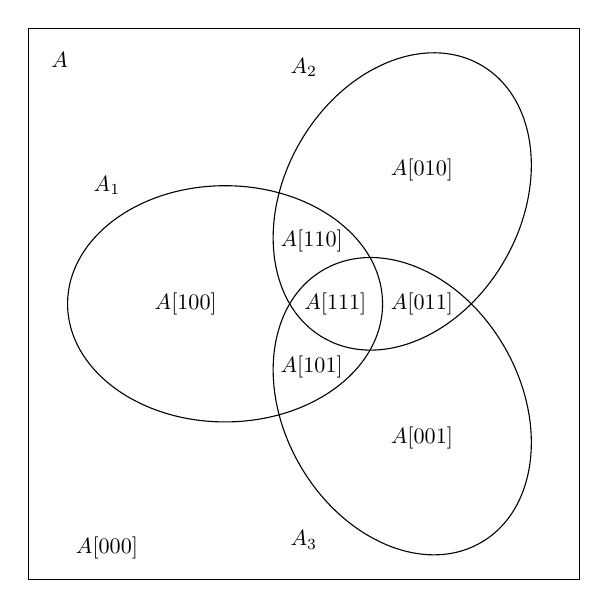
\begin{tikzpicture}
\draw (0,0) -- (7, 0) -- (7,7) -- (0,7) -- cycle;
\draw (2.5, 3.5) circle [x radius=2cm, y radius=1.5cm, rotate=0];
\draw (4.75, 4.8) circle [x radius=2cm, y radius=1.5cm, rotate=240];
\draw (4.75, 2.2) circle [x radius=2cm, y radius=1.5cm, rotate=120];
\node[scale=0.8] at (0.4, 6.6) {$A$};
\node[scale=0.8] at (1, 5) {$A_{1}$};
\node[scale=0.8] at (3.5, 6.5) {$A_{2}$};
\node[scale=0.8] at (3.5, 0.5) {$A_{3}$};
\node[scale=0.8] at (1, 0.4) {$A[000]$};
\node[scale=0.8] at (2, 3.5) {$A[100]$};
\node[scale=0.8] at (5, 5.2) {$A[010]$};
\node[scale=0.8] at (5, 1.8) {$A[001]$};
\node[scale=0.8] at (3.6, 4.3) {$A[110]$};
\node[scale=0.8] at (5, 3.5) {$A[011]$};
\node[scale=0.8] at (3.6, 2.7) {$A[101]$};
\node[scale=0.8] at (3.9, 3.5) {$A[111]$};
\end{tikzpicture}
\end{center}

\begin{lemma} \label{sequence of sets with half the measure}
Let $\mu:\m{A} \to \R^{m}$ be a semi-convex vector measure. For each $A\in \m{A}$ there exists a sequence $\{A_{i}\}_{i\in \N}$ from $\m{A}$ of subsets of $A$, so that for all $k\in \N$, any $k$ different integers, $1 \le n_{1} < \dots < n_{k}$ and any binary number $b\in B_{k}$,
\begin{align}
	\mu\left( \bigcap_{i=1}^{k} A_{n_{i}}^{b_{i}} \right) = \frac{1}{2^{k}} \mu(A) \label{eq: repeated semi-convexity}
\end{align}
\end{lemma}
\begin{proof}
 We can, by the semi-convexity of $\mu$, choose $A_{1}\subseteq A$, $A_{1}\in \m{A}$ so that $\mu(A_{1})=\frac{1}{2}\mu(A)$, and hence \eqref{eq: repeated semi-convexity} holds for $n_{1}=k=1$.

Now assume that $A_{1}, \dots, A_{n}$ has been chosen so that \eqref{eq: repeated semi-convexity} holds for all $k$ integers less than $n$, $1\le n_{1} < \dots < n_{k}\le n$ (note that $k \le n$ always). We will expand this solution by addition of a new set $A_{n+1}$ defined shortly: For each binary number $b\in B_{n}$ write
\begin{align*}
	A[b] := \bigcap_{i=1}^{k} A_{i}^{b_{i}}
\end{align*}
\emph{we note that $\mu(A[b])=\frac{1}{2^{k}}\mu(A)$}.
By the semi-convexity of $\mu$, pick a measurable $F[b]\in \m{A}$ such that $F[b] \subseteq A[b]$ and $\mu(F[b])=\frac{1}{2}\mu(A[b])$.

\textbf{Claim:} \eqref{eq: repeated semi-convexity} holds for all $k$ integers less than $n+1$ if we define
\begin{align}
	A_{n+1}:=\bigcup_{b\in B_{n}} F[b]. \label{eq: A n plus one}
\end{align}
Now the assumption in the induction step assures \eqref{eq: repeated semi-convexity} for all $k$ integers less than $n$, so we must prove the claim for $1\le n_{1} < \dots < n_{k-1} \le n$, $n_{k}=n+1$ and all $b\in B_{k}$.

Let $b\in B_{k}$ be given, and define
\begin{align*}
	\tilde{B}=\{c \in B_{n} | \forall i \in \{ 1, \dots, k-1 \} : c_{n_{i}} = b_{i}  \}
\end{align*}
which has exactly $2^{n-k+1}$ elements, since $k-1$ elements have already been chosen from $b$, and the rest is either 0 or 1.

%$\tilde{B}$ carries the information of the $n$ sets, $A_{1}, \dots, A_{n}$ while $b$ only carries the $k$ different sets $A_{n_{1}}, \dots, A_{n_{k}}$. So when we range over all $A[c]$, $c \in \tilde{B}$ we get the information of the parts of the partition of the sets $A_{1}, \dots, A_{n}$, which are included in all of the sets (in the intersection) of $A_{n_{1}}^{b_{1}}, \dots, A_{n_{k-1}}^{b_{k-1}}$. 
Observe that
\begin{align*}
	\bigcap_{i=1}^{k-1} A_{n_{i}}^{b_{i}} = \bigcup_{c\in \tilde{B}} A[c]
\end{align*}
If $b_{k}=1$,
\begin{align*}
	\bigcap_{i=1}^{k} A_{n_{i}}^{b_{i}} = \left( \bigcup_{c\in \tilde{B}} A[c] \right) \cap \left( \bigcup_{b\in B_{n}}F[b] \right) = \bigcup_{c\in \tilde{B}} F[c]
\end{align*}
where the first equality follows from \eqref{eq: A n plus one}, and the second equality follows from the fact that for all $b' \in B_{n}$, $b' \neq b$ where $b$ was the one we were given, $E[c] \cap F[b']=\emptyset$.

And if $b_{k}=0$,
\begin{align*}
	\bigcap_{i=1}^{k} A_{n_{i}}^{b_{i}} = \left( \bigcup_{c\in \tilde{B}} A[c] \right) \setminus \left( \bigcup_{b\in B_{n}}F[b] \right) = \bigcup_{c\in \tilde{B}} (A[c] \setminus F[c])
\end{align*}
because of the same argument as above.

In both cases, since $\mu(F[c])=\frac{1}{2}\mu(A[c])$, we get
\begin{align*}
	\mu\left( \bigcap_{i=1}^{k} A_{n_{i}}^{b_{i}} \right) &= \frac{1}{2} \sum_{c\in \tilde{B}} \mu(A[c]) \\
	&=\frac{1}{2}\frac{1}{2^{n}} \sum_{c\in \tilde{B}} \mu(A) \\
	&= \frac{1}{2}\frac{1}{2^{n}}2^{n-k+1}\mu(A)=\frac{1}{2^{k}}\mu(A)
\end{align*}
\end{proof}

This leads us to the following.

%%%%%%%%%%%%%%%%     %%%%%%%%%%%%%%%%

\begin{lemma}\label{thm: semi-convex implies convex}
A semi-convex measure $\mu:\m{A} \to \R^{n}$ is convex.
\end{lemma}
\begin{proof}
Let $A\in \m{A}$ be given, and choose $\{A_{i}\}_{i\in \N}$ from \Cref{sequence of sets with half the measure}.
Define
\begin{align*}
	A_{*}=\lim \inf_{n} A_{i} = \bigcup_{i\ge 1} \bigcap_{p\ge 0} A_{i+p},
\end{align*}
i.e. $x\in A_{*}$ if $x\in A_{i}$ eventually. Define
\begin{align*}
	\varphi(x)=\left( \sum_{i=1}^{\infty} \frac{1}{2^{i}}\mathbbm{1}_{A_{i}} \right) \cdot \mathbbm{1}_{A\setminus A_{*}}(x)
\end{align*}
This function is obviously well-defined and measurable, and $\varphi(X) \subseteq [0,1)$.
We will prove that $\varphi\in K(\mu, A)$. For a dyadic number $\frac{k}{2^{n}}$, $k\in \{1, \dots, 2^{n} \}$ we see that
\begin{align*}
	\left\{ \varphi(x) < \frac{k}{2^{n}} \right\} = A_{*} \cup \left\{ \sum_{i=1}^{n} \frac{1}{2^{i}}\mathbbm{1}_{A_{i}}(x) < \frac{k}{2^{n}} \right\}
\end{align*}
The direction ``$\subseteq$'' is clear.
For the other inclusion, if an $x$ is in the rightmost set, but $x\not\in A_{*}$ we must have
\begin{align*}
	\sum_{i=1}^{n}\frac{1}{2^{i}}\mathbbm{1}_{A_{i}}(x)\le \frac{k-1}{2^{n}}<\frac{k}{2^{n}}
\end{align*}
Since the inequality is strict in the rightmost set, and the sum must have the form $\frac{l}{2^{n}}$. Since $x\not\in A_{*}$ the following inequality is strict
\begin{align*}
	\sum_{i=n+1}^{\infty} \frac{1}{2^{i}}\mathbbm{1}_{A_{i}}(x) < \frac{1}{2^{n}},
\end{align*}
hence for such an $x$, $\varphi(x) < \frac{k-1}{2^{n}}+\frac{1}{2^{n}}=\frac{k}{2^{n}}$.

Now define
\begin{align*}
	B^{*}=\left\{b\in B_{n} \middle| \sum_{i=1}^{n} 2^{n-i}b_{i} < k \right\}
\end{align*}
which is just all the binary numbers, which when translated to base 10 is less than $k$. So $B^{*}$ has exactly $k$ elements. Using techniques from earlier, we see that
\begin{align*}
	\left\{ \sum_{i=1}^{n} \frac{1}{2^{i}} \mathbbm{1}_{A_{i}} < \frac{k}{2^{n}} \right\} = \left\{ \sum_{i=1}^{n} 2^{n-i} \mathbbm{1}_{A_{i}} < k \right\} = \bigcup_{b\in B^{*}} A[b]
\end{align*}
From \eqref{eq: repeated semi-convexity} above, it is clear that $A^{*}$ has measure zero, and that
\begin{align}
	\mu\left( \left\{ \varphi < \frac{k}{2^{n}} \right\} \right) &= \mu\left( \left\{ \sum_{i=1}^{n} \frac{1}{2^{i}}\mathbbm{1}_{A_{i}} < \frac{k}{2^{n}} \right\} \right) = \mu\left( \bigcup_{b\in B^{*}} A[b] \right) \nonumber \\
	&= \sum_{b\in B^{*}} \mu(A[b]) = \sum_{b\in B^{*}} \frac{1}{2^{n}} \mu(A) = \frac{k}{2^{n}}\mu(A). \label{eq: almost convex}
\end{align}
Now any $\alpha\in (0,1]$ is a limit of an increasing sequence, $\alpha_{i}$ of dyadic numbers, so since $\mu$ is countably additive and from the above calculations, we get
\begin{align*}
	\mu( \{ \varphi < \alpha \} ) = \mu\left( \bigcup_{i=1}^{\infty} \{ \varphi < \alpha_{i} \} \right) = \lim_{i\to \infty} \mu( \{ \varphi < \alpha_{i} \} ) \underset{\eqref{eq: almost convex}}{=} \lim_{i\to \infty} \alpha_{i}\mu(A) = \alpha \mu(A)
\end{align*}
Hence $\varphi\in K(\mu, A)$ as wanted.
\end{proof}

So a measure is semi-convex if and only if it is convex. Since semi-convexity is an easier concept to grasp, we will mostly be working with this.

%%%%%%%%%%%%%%%%     %%%%%%%%%%%%%%%%

\begin{lemma}\label{lem: continuous map from measure}
Let $\mu : \m{A} \to \R^{n}$ be a convex and non-negative vector measure, and let $A \in \m{A}$, $\varphi \in K(\mu, A)$. If $\nu: \m{A} \to \R^{m}$ is a vector measure and $\nu \ll \mu$, then the function $N:[0,1] \to \R^{n}$, given by
\begin{align*}
	N(\alpha) = \nu(\{\varphi < \alpha\})
\end{align*}
is continuous.
\end{lemma}
\begin{proof}
Each component $\nu_{i}$ of $\nu$ satisfies $\nu_{i}\ll \nu \ll |\mu|$. From $n$ applications of theorem \cref{thm: why it is called absolutely continuous} we get (using that $\mu$ is non-negative, hence $|\mu|(B)=\n{\mu(B)}_{1}$), that
\begin{align*}
	\forall \varepsilon > 0, \exists \delta > 0 \forall B\in \m{A}: \n{\mu(B)}_{1} < \delta \Rightarrow \n{\nu(B)}_{1} < \varepsilon
\end{align*}
so for $\varepsilon > 0$ given, if $|\alpha_{1}-\alpha_{2}| < \frac{\delta}{\n{\mu(A)}_{1}}$ with $\delta$ from above and $\alpha_{2}\le \alpha_{1}$, we have
\begin{align*}
	\n{\mu(\alpha_{2} \le \varphi < \alpha_{1} )}_{1} &= \n{ \mu(\varphi < \alpha_{1}) - \mu(\varphi < \alpha_{2}) }_{1} \\
	& = \n{ \alpha_{1}\mu(A) - \alpha_{2}\mu(A) }_{1} < \delta
\end{align*}
With this
\begin{align*}
	\n{N(\alpha_{1})-N(\alpha_{2})}_{1} &= \n{ \nu(\varphi < \alpha_{1}) - \nu(\varphi< \alpha_{2}) }_{1} \\
	&= \n{ \nu(\alpha_{2} \le \varphi < \alpha_{1}) }_{1} < \epsilon
\end{align*}
\end{proof}

%%%%%%%%%%%%%%%%     %%%%%%%%%%%%%%%%

The following theorem shows that a convex measure has convex range, however the example following the theorem shows that the converse is not true. However under certain assumptions the converse is true, and it is this theorem that we are working our way to prove.

\begin{theorem}\label{thm: why called convex}
Let $\mu: \m{A} \to \R^{n}$ be a convex vector measure, and $A, B \in \m{A}$. There exists a family $\{ C(\alpha) | \alpha \in [0,1] \} \subseteq \m{A}$ such that
\begin{itemize}
\item[(1)] $C(0)=A, C(1)=B$,
\item[(2)] $\mu(C(\alpha)) = \alpha\mu(A) + (1-\alpha) \mu(B)$.
\end{itemize}
Moreover, if $\mu$ is non-negative and $\nu \ll \mu$ then
\begin{itemize}
\item[(3)] $\alpha \mapsto \nu(C(\alpha))$ is continuous.
\end{itemize}
In particular, the range of a convex measure is convex.
\end{theorem}
\begin{proof}
Let $\varphi \in K(\mu, A \setminus B)$, $\psi \in K(\mu, B\setminus A)$ and define
\begin{align*}
	C(\alpha) = (A \cap B) \cup \{\varphi < 1-\alpha\} \cup \{\psi < \alpha\}  \quad \alpha \in [0,1]
\end{align*}
then $(1)$ follows by definition and $(3)$ follows from \Cref{lem: continuous map from measure}. To prove $(2)$ we see that
\begin{align*}
	\mu(C(\alpha))&=\mu(A\cap B) + \mu(\{\varphi<1-\alpha\}) + \mu(\{\psi<\alpha\}) \\
	&=\mu(A\cap B) + (1-\alpha)\mu(A\setminus B) + \alpha\mu(B\setminus A) \\
	&=(1-\alpha)[\mu(A\cap B) + \mu(A\setminus B)] + \alpha[\mu(A\cap B)+\mu(B\setminus A)] \\
	&=(1-\alpha)\mu(A)+\alpha\mu(A).
\end{align*}
as wanted.
\end{proof}

\begin{example}\label{convex range but not convex}
A vector measure with convex range, is not necessarily convex in the measure sense. We give a counterexample on $(\N, \m{P}(\N))$: 

Let $\tau$ be the counting measure, and let $f(n)=\frac{1}{n}$, for $n\in \N$. If we let $d\mu:=fd\tau$ (measure with density), i.e.
\begin{align*}
	\mu(A)=\sum_{n\in A}f(n), \qquad A\subseteq \N
\end{align*}
then $\mu$ is a finite measure that has convex range, but every singleton is an atom with respect to $\mu$.

We will later see, that with some restrictions on $\mu$, a vector measure will become convex.
\end{example}


%%%%%%%%%%%%%%%%   ATOMS   %%%%%%%%%%%%%%%%

\subsection{Atomic Sets}

\begin{definition}
Let $(X, \m{A}, \mu)$ be a measure space. A measurable set $A\in \m{A}$ is called an atom if
\begin{align*}
	&\mu(A)\neq 0 \\
	&\mu(B) \in \{0, \mu(A)\}, \quad \forall B\subseteq A, B\in \m{A}
\end{align*}
A vector measure, $\mu:(X,\m{A})\to \R^{n}$, is said to be \textbf{purely non-atomic} if none of the coordinate measures $\mu_{i}$ has any atoms. The measure is called \textbf{purely atomic}, if $\{A_{i}\}_{i\in I}$ is a countable family of disjoint sets that are atoms for all the coordinate measures, and such that
\begin{align*}
	X=\bigcup_{i\in I}A_{i}.
\end{align*}
\end{definition}

\begin{example}
The two measures in \cref{ex: selfmade examples} are purely non-atomic.

The Dirac measure $\delta_{x}$ on $(\R, \mathbb{B})$ has the atom $\{x\}$.

$X$ is an atom for every non-zero measure on the minimal $\sigma$-algebra, $\{\emptyset, X\}$.
\end{example}

Recall that for any $B\subseteq X$ and any $\sigma$-algebra $\m{A}$ in $X$,
\begin{align*}
	\m{A}_{B}:=\{B\cap A|A\in \m{A}\}
\end{align*}
is a $\sigma$-algebra called the trace $\sigma$-algebra.

Because of the following discussion, a purely non-atomic measure could be thought of as a measure that is ``strongly'' convex.

Let $(X, \m{A}, \mu)$ be a measure space. Then the measure $\mu$ is convex with respect to every trace $\sigma$-algebra on $\m{A}$ if and only if $\mu$ is purely non-atomic. The first implication, ``$\Rightarrow$'', is quite easy, because for every $B\in \m{A}$, the measure, $\mu|_{\m{A}_{B}}$, restricted to $\m{A}_{B}$ is convex, hence there exists a $C\in \m{A}$ such that $\mu|_{\m{A}_{B}}(B\cap C)=\frac{1}{2}\mu|_{\m{A}_{B}}(B)$ as wanted. The other inclusion is quite difficult though, but will be a direct consequence of Liapunoff's convexity theorem proven later.

We will shortly prove Liapunoff's convexity theorem, but we need the following Lemma, which is a finite version of the convexity theorem for ordinary measures.

\begin{lemma}\label{lem: finite liapunoff}
A purely non-atomic, finite, positive measure $\mu:\m{A}\to [0,\infty)$ is convex.
\end{lemma}
\begin{proof}
By \cref{thm: semi-convex implies convex} it is enough to prove semi-convexity.

For an $A\in \m{A}$ we must find a $B\in \m{A}$, with $B\subseteq A$ such that
\begin{align*}
	\mu(B)=\frac{1}{2}\mu(A)
\end{align*}
We may assume that $\mu(A)\neq 0$. For any $\alpha\in (0,1)$ there exists a $B_{\alpha}\subseteq A$, $B_{\alpha}\in \m{A}$ such that
\begin{align}
	0< \mu(B_{\alpha}) \le \alpha\mu(A) \label{eq: B alpha}
\end{align}
If $\alpha< 2^{-n}$ the inequality follows from $n$ applications of the fact that $\mu$ is purely non-atomic, so that every measurable set $A\in \m{A}$ with positive measure has a partition $\{A_{1}, A_{2}\}$ such that $\mu(A)=\mu(A_{1})+\mu(A_{2})$ with both $\mu(A_{i})>0$, $i=1,2$. Hence every measurable set contains a subset with at most half the measure.

If $\{A_{i}|i\in I, \mu(A_{i})>0\}$ is a family of disjoint sets, then the index set $I$ must be countable. Indeed each of the sets
\begin{align*}
	I_{n}:=\left\{i\in I | \mu(A_{i}) > \frac{1}{n} \right\}
\end{align*}
are finite since $\mu(X)<\infty$ and $I=\bigcup_{1}^{\infty}I_{n}$. So since $I$ is countable, $\bigcup_{I}A_{i}\in \m{A}$.

We will call a family $\m{E}\subseteq \m{A}$ disjoint if it consists of mutually disjoint sets. Furthermore we define
\begin{align*}
	\mathbb{E}:=\left\{ \m{E}\subseteq \m{A} \middle| \m{E} \text{ disjoint }, \forall E\in \m{E} (E\subseteq A, \mu(E)>0), \mu\left( \bigcup_{E\in \m{E}} E\right) \le \frac{1}{2}\mu(A) \right\}
\end{align*}
$\mathbb{E}$ is inductively ordered\footnote{Every totally ordered subset (chain) of $\mathbb{E}$ has a least upper bound.} by inclusion. Since if $\{\m{E}_{j}\}_{j\in J}$ is a chain in $\mathbb{E}$, then
\begin{align*}
	\m{E}:=\bigcup_{j\in J}\m{E}_{j}
\end{align*}
is a majorant for $\{\m{E}_{j}\}_{j\in J}$. We must prove that $\m{E}\in \mathbb{E}$ before we can say that $\mathbb{E}$ is inductively ordered. So if $E_{1},E_{2}\in \mathbb{E}$ there exists $j_{1},j_{2}\in J$ such that $E_{1}\in \m{E}_{j_{1}}$ and $E_{2}\in \m{E}_{j_{2}}$, where we assume by the total ordering of $\m{E}$ that $\m{E}_{j_{1}} \supseteq \m{E}_{j_{2}}$, so that $E_{1}$ and $E_{2}$ are disjoint if they are different.

By the discussion above (about the family $I$), $\m{E}$ must be countable, so we write $\m{E}=\{E_{1}, E_{2}, \dots\}$. For some $j_{n}\in J$ we have $\{E_{1}, \dots, E_{n}\}\subseteq \m{E}_{j_{n}}$, and therefore from the definition of $\mathbb{E}$
\begin{align*}
	\mu\left( \bigcup_{i=1}^{n}E_{i} \right) \le \frac{1}{2}\mu(A)
\end{align*}
Since $\mu$ is countably additive, the inequality holds for all $\{E_{1}, E_{2}, \dots\}$ as well:
\begin{align*}
	\mu\left( \bigcup_{i=1}^{\infty}E_{i} \right) = \sum_{i=1}^{\infty}\mu(E_{i}) = \lim_{n\to \infty}\sum_{i=1}^{n}\mu(E_{i})=\lim_{n\to \infty} \mu\left( \bigcup_{i=1}^{n} E_{i} \right) \le \frac{1}{2} \mu(A)
\end{align*}
as required.

For a $B_{\alpha}$ chosen such that \eqref{eq: B alpha} holds for $\alpha \le \frac{1}{2}$, then $\{B_{\alpha}\}\in \mathbb{E}$ hence we can use Zorn's Lemma since then $\mathbb{E}$ is non-empty.

Choose $\m{E}_{0}=\{E_{i} | i\in I\}$ maximal from $\mathbb{E}$. For this set we must have
\begin{align*}
	\mu\left( \bigcup_{i\in I} E_{i} \right)=\frac{1}{2}\mu(A).
\end{align*}
If not, then
\begin{align*}
	\mu\left( \bigcup_{i\in I}E_{i} \right) \le \left( \frac{1}{2} - \alpha \right) \mu(A)
\end{align*}
hence we could find, since $\mu$ is purely non-atomic, some $B_{\alpha}\subseteq A\setminus \bigcup_{i}E_{i}$ such that $\mu(B_{\alpha})\le \alpha \mu(A)$. But then
\begin{align*}
	\m{E}_{0}\cup \{B_{\alpha}\} \in \mathbb{E}
\end{align*}
which would contradict the maximality of $\m{E}_{0}$.
\end{proof}



\begin{lemma}\label{lem: chain of ac}
Let $\mu=(\mu_{1}, \dots, \mu_{n}):\m{A}\to \R^{n}$ be a non-negative and purely non-atomic vector measure, and assume that
\begin{align}
	\mu_{i} \ll \mu_{i-1}, \quad i\in \{2, \dots, n \} \label{eq: absolutely continuous assumption}
\end{align}
then $\mu$ is convex.
\end{lemma}
\begin{proof}
The proof follows by induction on $n$. For an $A\in \m{A}$, we saw by \cref{thm: semi-convex implies convex} that it is enough to find a $B\in \m{A}, B\subseteq A$ such that $\mu(B)=\frac{1}{2}\mu(A)$.

For $n=1$, $B$ is given from \Cref{lem: finite liapunoff}. For $n>1$ assume $\mu'=(\mu_{1}, \dots, \mu_{n-1})$ is convex. For $\nu'=\mu_{m}$ we have by \eqref{eq: absolutely continuous assumption}, that $\nu' \ll \mu'$.
Since $\mu'$ is convex there exists a measurable $A_{0}\subseteq A$, $A_{0}\in \m{A}$ such that
\begin{align*}
	\mu'(A_{0})=\frac{1}{2}\mu'(A)
\end{align*}
If $\nu'(A_{0})=\frac{1}{2}\nu'(A)$ we are done, with $B=A_{0}$. If not, let $B_{0}=A\setminus A_{0}$ and assume that
\begin{align*}
	\nu'(A_{0})<\frac{1}{2}\nu'(A), \qquad \nu'(B_{0})>\frac{1}{2}\nu'(A).
\end{align*}
Using \cref{thm: why called convex}(iii) applied to $A_{0}, B_{0}, \mu',\nu'$, gives us a family $\{C(\alpha)|\alpha\in[0,1]\}$ and an $\alpha_{0}\in [0,1]$ such that
\begin{align*}
	\nu'(C(\alpha_{0}))=\frac{1}{2}\nu'(A)
\end{align*}
since $[0,1]$ is connected. Using \cref{thm: why called convex}(ii) we finally have
\begin{align*}
	\mu'(C(\alpha_{0}))&=(1-\alpha_{0})\mu'(A_{0})+\alpha_{0}\mu'(B_{0}) = \frac{1}{2}(1-\alpha_{0})\mu'(A_{0})+\frac{1}{2}\alpha_{0}\mu'(B_{0}) \\
	&=\frac{1}{2}\mu'(A)
\end{align*}
and putting $B=C(\alpha_{0})$ shows the (semi-)convexity.
\end{proof}

%%%%%%%%%%%%%%%%   Liapunoff's Convexity Theorem  %%%%%%%%%%%%%%%%
\subsection{Liapunoff's Convexity Theorem}

In 1940 Liapunov proved the following theorem along with \cref{thm: Liapunoff closed}. We will first prove them here using the measure theory we have developed so far, both the theory of vector measures and complex measures. The proofs are however not very elegant and together they are long. Later on, though, we will see another proof (\cref{thm: Lindenstrauss}) using tools from functional analysis, which proves both theorems in a much more short and elegant way.

\begin{theorem}[Lyapunov, 1940]\label{thm: Liapunoff convex}
A purely non-atomic vector measure $\mu: \m{A} \to \R^{n}$ is convex, and in particular the range $\mu(\m{A})$ is a convex subset of $\R^{n}$.
\end{theorem}
\begin{proof}
Again, it is enough to prove only semi-convexity of $\mu$.

1: First, let us assume that $\mu$ is non-negative. The vector measure $\mu'$ given by
\begin{align*}
	\mu'_{i}:=\sum_{j=i}^{n}\mu_{j}, \quad i=1, \dots, m
\end{align*}
is obviously purely non-atomic, and since it satisfies the conditions of \Cref{lem: chain of ac}, because
\begin{align*}
	\mu'_{i}=\sum_{j=i}^{n}\mu_{j} \le \sum_{j=i-1}^{n}\mu_{j} = \mu'_{i-1},
\end{align*}
it is also convex. For the upper triangle matrix
\begin{align*}
	T:=\begin{bmatrix}
	1 & 1 & \dots & 1 & 1 \\
	0 & 1 & \dots & 1 & 1 \\
	\vdots & \vdots &  & \vdots & \vdots \\
	0 & 0 & \dots & 0 & 1 \\
	\end{bmatrix}
\end{align*}
we have $\mu'=T\mu$. Now $T$ is invertible, and since $\mu'$ is (semi-)convex, we have for each $A\in \m{A}$, some $B\subseteq A$, $B\in \m{A}$ satisfying $\mu'(B)=\frac{1}{2}\mu'(A)$, and therefore
\begin{align*}
	\mu(B)=T^{-1}\mu'(B)=T^{-1}\left(\frac{1}{2}\mu'(A)\right) = \frac{1}{2}T^{-1}\mu'(A)=\frac{1}{2}\mu(A).
\end{align*}

2: When $\mu$ is \emph{any} purely non-atomic vector measure, we consider the measure
\begin{align*}
	\mu''=(\mu_{1}^{+}, \mu_{1}^{-}, \dots, \mu_{n}^{+}, \mu_{n}^{-}).
\end{align*}
%%%%%%% Where are the positive and negative parts defined...
By definition, $\mu''$ is non-negative, and the Hahn decomposition theorem gives us partitions $\{P_{i}, N_{i}\}_{1\le i \le n}$ of $X$ such that
\begin{align*}
	\mu_{i}^{+}(B)=\mu_{i}(B\cap P_{i}), \qquad \mu_{i}^{-}(B)=-\mu_{i}(B\cap N_{i}).
\end{align*}
Hence an atom of $\mu_{i}^{+}$ or $\mu_{i}^{-}$ would also be an atom of $\mu_{i}$. Thus $\mu''$ is purely non-atomic, and for any $A\in \m{A}$, part 1 of this proof gives us a $B\subseteq A$, $B\in \m{A}$ such that $\mu''(B)=\frac{1}{2}\mu''(A)$. But this gives us
\begin{align*}
	\mu(B)&=(\mu_{1}^{+}(B) - \mu_{1}^{-}(B), \dots, \mu_{n}^{+}(B) - \mu_{n}^{-}(B)) \\
	&=\frac{1}{2}(\mu_{1}^{+}(A) - \mu_{1}^{-}(A), \dots, \mu_{n}^{+}(A) - \mu_{n}^{-}(A)) \\
	&=\frac{1}{2}\mu(A)
\end{align*}
as wanted.
\end{proof}

%%%%%%%%%%%%%%%%   Closed range  %%%%%%%%%%%%%%%%

\subsection{Liapunoff's Closed Range Theorem}

%%%%%%%%%%%%%%%%   Hyperplane  %%%%%%%%%%%%%%%%
For the remaining pages in this chapter, we will develop the theory to prove \cref{thm: Liapunoff closed} which says that the range of a vector measure is closed. When dealing with closed and convex sets in $\R^{n}$ we will turn to the notion of supporting hyperplanes.

\begin{definition}
A hyperplane $H$ \textbf{supports} the closed convex set $A$, when $A\cap H\neq \emptyset$ and $A$ is contained in one of the two closed half-spaces bounded by $H$.

A hyperplane $H$ has the form $\{x\in \R^{n}|\varphi(x) = \alpha \}$ for some (continuous) linear functional $\varphi: \R^{n} \to \R$. We may assume (if necessary, replacing $(\alpha, \varphi)$ with $(-\alpha, -\varphi)$) that $\varphi(A)\subseteq [\alpha, \infty)$.
A set has many different supporting hyperplanes, as illustrated in the picture:
\begin{center}
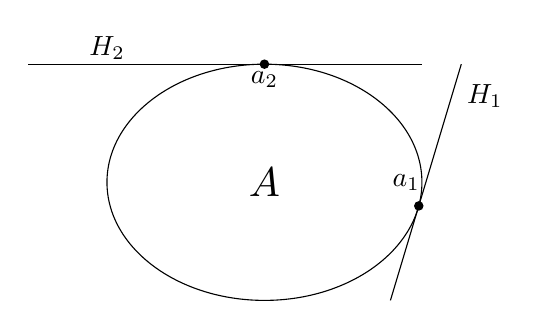
\begin{tikzpicture}
\draw (-3, 1.5) -- (2, 1.5);
\draw (1.6, -1.5) -- (2.5, 1.5);
\draw (0, 0) circle [x radius=2cm, y radius=1.5cm, rotate=0];
\node[scale=1.5] at (0, 0) {$A$};
\node at (0, 1.3) {$a_{2}$};
\node at (-2, 1.7) {$H_{2}$};
\filldraw[fill=black, draw=black] (0, 1.5) circle (1.5pt);
\node at (1.8, 0) {$a_{1}$};
\node at (2.8, 1.1) {$H_{1}$};
\filldraw[fill=black, draw=black] (1.96, -0.3) circle (1.5pt);
\end{tikzpicture}
\end{center}
\end{definition}

\begin{theorem}\label{thm: hyperplane}
If $A$ is a closed convex set in $\R^{n}$ and $a\in \partial A$, there is a supporting hyperplane $H$ of $A$ such that $a\in H$.
\end{theorem}
\begin{proof}
See \cite{Brondsted82}: Arne Brøndsted: An introduction to convex polytopes, theorem 4.3.
\end{proof}

\begin{lemma}\label{lem: non-empty hyperplane cap}
If a vector measure $\mu:\m{A}\to \R^{n}$ has convex range $R:=\mu(\m{A})$ and $H$ is a supporting hyperplane of $\overline{R}$, then $H\cap R \neq \emptyset$.
\end{lemma}
\begin{proof}
Let $H=\{x\in \R^{n} | \varphi(x) = \alpha \}$ and $\overline{R}\subseteq \{x\in \R^{n} | \varphi(x) \ge \alpha\}$. Since by definition $H\cap \overline{R}\neq \emptyset$, hence
\begin{align*}
	\alpha=\inf\{ \varphi(\mu(A)) | A \in \m{A} \}.
\end{align*}
So if we write $\varphi$ as $\varphi=\sum_{i=1}^{n}a_{i}x_{i}$, then $\varphi\circ\mu=\sum_{i=1}^{n}a_{i}\mu_{i}$ is a real measure.

As a consequence of Hahn's decomposition theorem this measure $\varphi \circ \mu$ attains its minimum. In the decomposition theorem, this minimum us realized by $N$.
Therefore $\alpha\in \varphi\circ \mu(\m{A})=\varphi(R)$ as wanted.
\end{proof}

\begin{lemma}\label{lem: shifted measure}
If $\mu:\m{A} \to \R^{n}$ is a vector measure with range $R$ and $x_{0}\in R$, there exists a vector measure $\mu'$ with range $R'=R-x_{0}:=\{r-x_{0} | r\in R\}$. If $\mu$ is convex, then so is $\mu'$.
\end{lemma}
\begin{proof}
With $x_{0}=\mu(B)$ for some $B\in \m{A}$ put
\begin{align}
	\mu'(A)=\mu(A\setminus B) - \mu(A\cap B), \quad A\in \m{A}. \label{eq: shifted range def}
\end{align}
Now $\mu'$ is a vector measure, and
\begin{align*}
	\mu'(A)=\mu(A\setminus B) - (\mu(B) - \mu(B\setminus A)) = \mu((A\setminus B) \cup (B\setminus A)) - x_{0}
\end{align*}
hence $R':=\mu'(\m{A})\subseteq R-x_{0}$. For the other inclusion, we see that
\begin{align*}
	\mu(A)-x_{0}&=\mu(A)-\mu(B)=\mu(A\setminus B) - \mu(B\setminus A) \\
	&=\mu'((A\setminus B) \cup (B\setminus A)),
\end{align*}
where the last equality follows from \eqref{eq: shifted range def} used on $(A\setminus B) \cup (B\setminus A)$. With this $R-x_{0}\subseteq R'$, so equality holds.

If $\mu$ is convex, we can for a given $A\in \m{A}$ choose $F^{-}, F^{+}\in \m{A}$ such that
\begin{align*}
	F^{-}\subseteq A\setminus B, \qquad \mu(F^{-})=\frac{1}{2}\mu(A\setminus B), \\
	F^{+}\subseteq A\cap B, \qquad \mu(F^{+})=\frac{1}{2}\mu(A\cap B).
\end{align*}
Applying \eqref{eq: shifted range def} to $F^{-}$ and $F^{+}$ we get (since $F^{-}\cap B=\emptyset$ and $F^{+}\subseteq B$), that
\begin{align*}
	\mu'(F^{-})=\mu(F^{-}), \qquad \mu'(F^{+})=-\mu(F^{+})
\end{align*}
and hence
\begin{align*}
	\mu'(F^{-}\cup F^{+})=\mu(F^{-})-\mu(F^{+})=\frac{1}{2}(\mu(A\setminus B) - \mu(A\cap B))=\frac{1}{2}\mu'(A)
\end{align*}
so $\mu'$ is (semi-)convex.
\end{proof}

\begin{definition}
An \textbf{affine (sub-)space} of $\R^{n}$ is either $\emptyset$ or a subset $A=x+L\subseteq \R^{n}$ with $x\in \R^{n}$ where $L$ is a linear subspace of $\R^{n}$.

The dimension $\dim(A)$ of a non-empty affine space is the dimension of the linear subspace $L$ such that $A=x+L$. The space $L$ can be shown to be unique, hence the dimension is well-defined. If $A$ is itself a linear subspace, then the affine and the linear dimensions coincide, hence the abuse of notation. If $A=\emptyset$, we define $\dim(A)=-1$. In the following Lemma, the affine dimension will refer to the affine dimension of the smallest affine space containing the original space. This space is defined as the intersection of all affine spaces containing the space, and is itself an affine subspace.
\end{definition}

\begin{lemma}\label{lem: convex means closed}
The range of a convex vector measure $\mu:\m{A}\to \R^{n}$ is closed.
\end{lemma}
\begin{proof}
The proof follows by complete induction on the affine dimension, $m$, of $R:=\mu(\m{A})$, i.e. the dimension of the smallest affine space containing $R$, as discussed above.

For $m=1$, the range is a linear subspace in $n$-dimensional space, so $\mu$ has the form
\begin{align*}
	\mu(A)=\xi \mu_{0}(A), \quad A\in \m{A}
\end{align*}
for some $\xi\in \R^{n}$ and some (finite) real measure, $\mu_{0}$. Since $R$ is convex, $\mu_{0}(\m{A})$ is an interval of $\R$, which is closed since real measures attain their extrema.

When $m>1$ we assume that the range of convex vector measures with affine dimension less than $m$ are closed.
With this assumption we will show that for every supporting hyperplane $H$ of $\overline{R}$, it holds that $H\cap R\subseteq R$. It will then follow from \cref{thm: hyperplane} that $\partial(\overline{R})\subseteq R$, but for convex sets in $\R^{n}$ it is known that $\partial(\overline{R})=\partial(R)$, and it thus follows that $R$ is closed.

From \Cref{lem: non-empty hyperplane cap} there exists an element $x_{0}\in R\cap H$, and from \Cref{lem: shifted measure} we know that $R-x_{0}$ is also the range of a convex measure, therefore we may assume that $0\in H$ (we can just replace $R,H,\mu$ by their shifted versions: $R-x_{0},H-x_{0},\mu'$, where $\mu'$ is as given in \Cref{lem: shifted measure}).

Take a bounded linear functional, $\varphi$, such that $H=\{\varphi(x)=0\}$ and $\overline{R}\subseteq \{ \varphi(x) \ge 0\}$. Then $\nu=\varphi\circ \mu$ is a positive measure %%%%% from where
and the Lebesgue decomposition gives us, for each coordinate measure $\mu_{i}$, a partition $\{A_{i}, S_{i}\}$ such that letting
\begin{align*}
	\mu_{i}^{a}(B)=\mu_{i}(A_{i}\cap B), \quad \mu_{i}^{s}(B)=\mu_{i}(S_{i}\cap B), \qquad B\in \m{A}
\end{align*}
with
\begin{align*}
	\mu_{i}^{a} \ll \nu, \quad \mu_{i}^{s} \perp \nu, \quad \nu(S_{i})=0
\end{align*}
from the proof of the Lebesgue-Radon-Nikodym theorem.
Writing
\begin{align*}
	S=\bigcup_{i=1}^{n}S_{i}, \quad A=X\setminus S
\end{align*}
and
\begin{align*}
	\mu_{A}(B)=\mu(B\cap A), \quad \mu_{S}=\mu(B\cap S), \quad B\in \m{A}
\end{align*}
we have $\mu=\mu_{A}+\mu_{S}$ and since $A\subseteq A_{i}$, $i=1,\dots, n$, we have
\begin{align*}
	\mu_{A} \ll \nu, \quad \nu(S)=0.
\end{align*}
With $R_{S}:=\mu_{S}(\m{A})$ then $R_{S}\subseteq H$ since
\begin{align*}
	\varphi(\mu_{S}(B)) = \nu(B\cap S) = 0.
\end{align*}
The vector measure $\mu_{S}$ is clearly (semi-)convex, and since the dimension of $R_{S}$ is at most $m-1$ we have by the induction hypothesis that $R_{S}$ is closed.

Now with $x_{0}\in \overline{R}\cap H$, there exists a sequence $\{B_{i}\}_{i\in \N}\subseteq \m{A}$, such that $\mu(B_{i})\to x_{0}$, for $i\to \infty$, and for this sequence $\nu(B_{i})\to \varphi(x_{0})=0$ for $i\to \infty$. Since $\mu_{A} \ll \nu$ we get from \cref{thm: why it is called absolutely continuous},
that $\mu_{A}(B_{i})\to 0$, $i\to \infty$, and therefore
\begin{align*}
	x_{0}=\lim_{i\to \infty} \mu(B_{i})=\lim_{i\to \infty} (\mu_{A}(B_{i}) + \mu_{S}(B_{i})) = \lim_{i\to \infty} \mu_{S}(B_{i}) \in \overline{R_{S}}=R_{S}\subseteq R.
\end{align*}
as wanted.
\end{proof}


Now to the last part of Liapunoff's theorem.

\begin{theorem}[Lyapunov, 1940]\label{thm: Liapunoff closed}
The range of a vector measure $\mu:\m{A}\to \R^{n}$ is closed.
\end{theorem}
\begin{proof}
1: Let $M$ be an $n\times n$-matrix with positive entries, then replacing $\mu$ by $M\circ \mu$ gives us a vector measure, where every coordinate measure is absolutely continuous with respect to every other. We see that the common null-sets are the sets $A\in \m{A}$ for which $\mu_{i}(A)=0$, for all $i=1, \dots, n$. If the range of $M\circ \mu$ is closed, so is the range of $\mu$ since $M$ is a homeomorphism in the topological sense (i.e. a bijective and continuous map with continuous inverse).
We can thus assume that $\mu$ also has this property of mutual absolute continuity of the components like $M\circ \mu$. In particular, every atom of a coordinate of $\mu$ is an atom of every other.

Since a $\sigma$-algebra is closed under countable union, every countable chain of atoms has their countable union as an upper bound, hence we can use Zorn's Lemma.
So from a Zorn's Lemma argument we can choose a maximal family $\{A_{i}\}_{i\in I}$ of disjoint common atoms. Since $\mu_{j}(A_{i})>0$ for every $i,j$, and since vector measures are finite, we see that $I$ is countable. With
\begin{align*}
	A:=\bigcup_{i\in I} A_{i}, \quad N:=X\setminus A
\end{align*}
we obtain a decomposition of $\mu$, namely
\begin{align*}
	\mu_{A}(B)=\mu(B\cap A), \quad \mu_{N}(B)=\mu(B\cap N), \quad B\in \m{A}
\end{align*}
with $\mu_{A}$ purely atomic and $\mu_{N}$ purely non-atomic.
The range $R_{N}:=\mu_{N}(\m{A})$ is closed by \cref{thm: Liapunoff convex} and \Cref{lem: convex means closed}. Observe that
\begin{align*}
	\mu_{A}(B)=\mu\left( \bigcup_{i\in I} (A_{i} \cap B) \right) = \sum_{i\in I} \mu(A_{i}\cap B)=\sum_{i\in I} b_{i}(B)\mu(A_{i})
\end{align*}
with $b_{i}(B)\in \{0,1\}$, thus the range $R_{A}:=\mu_{A}(\m{A})$ can be written as
\begin{align*}
	R_{A}=\left\{ \sum_{i\in I} b_{i}\mu(A_{i}) | \{b_{i}\}_{i\in I} \in \{0,1\}^{I} \right\}.
\end{align*}
Equipped with the discrete metric, $\{0,1\}$ is compact, hence $\{0,1\}^{I}$ with the product topology is also compact by Tychonoff's theorem. %%%%%% INCLUDE THIS???.
The space $\{0,1\}^{I}$ is metrizable under the metric
\begin{align*}
	d(b,c)=\sum_{j=1}^{\infty}2^{-j}|c_{i_{j}} - b_{i_{j}}|,
\end{align*}
for some ordering $\{i_{1}, i_{2}, \dots\}$ of $I$. Define a map $\varphi:\{0,1\}^{I}\to \R^{n}$ by
\begin{align*}
	\varphi(b)=\sum_{i\in I} b_{i} \mu(A_{i}).
\end{align*}
Given $b\in \{0,1\}^{I}$ and $\varepsilon>0$, choose $j_{0}$ such that
\begin{align*}
	\sum_{j=j_{0}+1}|\mu(A_{i_{j}})|_{1}<\varepsilon.
\end{align*}
When $d(b,c)<2^{-j_{0}}$ then the first $j_{0}$ coordinates of $b$ and $c$ agree, and hence $| \varphi(b) - \varphi(c) |_{1} < \varepsilon$ so $\varphi$ is continuous.

This shows that $R_{A}=\varphi(\{0,1\}^{I})$ is compact, and since
\begin{align*}
	R=R_{A}+R_{N},
\end{align*}
$R$ is compact as well, hence it is closed.

2: In the general case, consider the vector measure
\begin{align*}
	\nu:=(\mu_{1}^{+}, \mu_{1}^{-}, \dots, \mu_{n}^{+}, \mu_{n}^{-}),
\end{align*}
which is non-negative with values in $\R^{2n}$, so its range is compact by part 1 of this proof. If we define the continuous map $f:\R^{2n}\to \R^{n}$ by
\begin{align*}
	f(x_{1},y_{1}, \dots, x_{n},y_{n}):=(x_{1}-y_{1}, \dots, x_{n}-y_{n})
\end{align*}
then $\mu(\m{A})=f(\nu(\m{A}))$ is also compact.
\end{proof}





